\documentclass[../manifest.tex]{subfiles}


% - describe your solution idiom, analyze it according to the framework of the book, and justify your design choices with respect to alternative possibilities
% - if you have done any significant algorithmic work, discuss the algorithm and data structures
% - you might choose to split out Interface into its own section

\begin{document}

In this section we describe our visualization solution and analyze it using the What-Why-How framework provided by \cite{Munzner:2014} for which table~\ref{tab:analysis} provides a summary.

\begin{table}
  \caption{What-Why-How analysis of Teamline.}
  \label{tab:analysis}
  \begin{tabularx}{\columnwidth}{ l | X }
    \hline
    What: Data & Table of graded commits with attributes described in \ref{tab:attributes}. \\
    \hline
    What: Derived & Measure of contribution to pass rate and coverage; contribution uniformity. These are discussed in section \ref{ssec:data-description}. \\
    \hline
    Why: Tasks & Present the uniformity of contributions and summarize the team's commit history. Identify teams with highly non-uniform contributions. \\
    \hline
    How: Encode & We used a heatmap with sparklines in the overview  and line charts in the detail view. Marks are positioned on a common time scale with color indicating the attribute that is being encoded.\\
    \hline
    How: Facet & Overview + detail views. Detail view is partitioned into side-by-side views. \\
    \hline
    How: Embed & Superimpose sparklines on the overview's heatmap cells. \\
    \hline
    How: Reduce & Filtering is done by selecting the team and the deliverable. \\
    \hline
  \end{tabularx}
\end{table}

Teamline is faceted into two views: an \textbf{overview} providing a summary for all teams and a \textbf{detail view} for each team. The content shown in both the overview and the detail view is filtered by using the controls above the charts, labelled \textit{D1}, \textit{D2}, and \textit{D3}, to indicate the corresponding deliverable. To filter by team, the user can select the corresponding heatmap cell in the overview of by updating the team number shown in the detail view.

\subsection{Overview}

The user is first presented the \textbf{overview} shown in figure~\ref{fig:sample-overview}\footnote{The highlighted cell is used in section~\ref{sec:results} and can be ignored for now.} which uses a heatmap to encode the within-team contribution uniformity where a higher saturation indicates a more uneven contribution distribution. We initially used red for the hue but later decided on orange because we considered red to be too negative. We chose a heatmap because it is able to accommodate the approximately 200 teams in a single view without needing to scroll. Showing the contribution of every team on a single page is important so that the user is able to quickly identify teams with one member contributing less than the others. To further increase the information density and utility of the overview, we embedded sparklines in the heatmap cells. Sparklines are an ideal choice in this instance because they show trends without the extra clutter of axes found in true line charts. However, they closely resemble line charts which helps maintain consistency with the detail view. We opted to use the same color as in the detail view both for consistency and because it contrasts well with all saturation levels of the heatmap cell. The sparklines help the user see how teams are progressing based on grade and, combined with the saturation, let the user quickly identify dysfunctional teams that warrant further investigation in the detail view.


  % of of teams (\textit{how: encode}) enriched with a sparkline in each cell (\textit{how: embed}). The major attribute we want to show is the \textit{Within-team contribution uniformity} (see section~\ref{sec:abstractions}) which is encoded by saturation of the team cells: low saturation indicates uneven contribution and high saturation indicates even distribution.
  %
  %  We chose a color-coding ranging from white (for most even contribution) to dark orange (for most uneven contribution). We discussed an alternative approach ranging from white for most uneven contribution to green for most even contribution (white = negative) but argued that TAs really aim to see at a glance what teams had uneven contribution and that a positive white and negative orange would highlight this aim better. We initially used a red color for uneven contribution but considered the appearance of the overview having a too negative overall connotation and switched to a 'warmer' orange color. The second attribute we were interested in for the overview of all teams was the \textit{progression of each team's grade}. We decided for a sparkline for each team that clearly indicates both the team's final grade and how the grade developed throughout the duration of the deliverable. The color of the sparklines matches the color of the grade line in the team view.

\subsection{Detail View}

Clicking on a heatmap cell switches to the \textbf{detail view} shown in figure~\ref{fig:sample-teamview}. The detail view is based on the team that was clicked on in the overview and can be changed on the fly by changing the team name in the menu bar which will result in redrawing operations of all charts. This view includes a stage area that is partitioned into three side-by-side views and a gallery area with a variable number of thumbnail line charts on the bottom. The stage area contains the \textbf{grade chart} (leftmost) and two \textbf{contribution charts} (middle and rightmost). All three charts share a common y-axis which encodes time. We chose this configuration, as opposed to using the x-axis to encode time, because version control systems commonly design their commit graphs that way and it allows us to take advantage of the wider screen aspect ratio of most modern consumer monitors. The x-axis is used to encode attribute values which differ based on the line chart. For the grade chart, the x-axis encodes the percentage pass rate, percentage coverage, and the overall percentage grade. The contribution charts encode the percentage contribution to pass rate and percentage contribution to coverage with the x-axis. To help us choose reasonable colors for the chart lines representing the five attributes, we used a 5-class qualitative color scale from Color Brewer\footnote{http://colorbrewer2.org/}.


%% why line charts?

%% Discuss the gallery







% We decided to encode time on the y-axis in all line charts because version control systems commonly design their commit graphs that way\footnote{Example: https://bestchai.bitbucket.io/shiviz/}. The value of the attributes shown in the line charts is encoded on the x-axis. We generally used Color Brewer\footnote{http://colorbrewer2.org/} for choosing the colors for our line charts
%
% The \textbf{grade chart} (left line chart on the stage) shows absolute values for the \textit{pass rate}, \textit{coverage} and \textit{grade} for the team. We considered the grade the most important attribute in this chart so we gave it the highest saturated color. Since the left chart is showing absolute values for the three attributes, we can often see lines switching between left and right which often indicates regression bugs and out- and uncommenting of lines between commits which can affect pass rate and coverage strongly.
%
% The \textit{contribution charts}... TODO
%
%
%
%
%
%
%
%  %%%%
% Clicking on a team cell switches to the \textbf{team view} (see figure~\ref{fig:sample-teamview}) which is divided in a stage area with three line charts and a gallery area with a variable number of thumbnail line charts on the bottom. The team view is based on the team that was clicked on in the overview. It can be changed on the fly by changing the team name in the menu bar which will result in redrawing operations of all charts. We decided to encode time on the y-axis in all line charts because version control systems commonly design their commit graphs that way\footnote{Example: https://bestchai.bitbucket.io/shiviz/}. The value of the attributes shown in the line charts is encoded on the x-axis. We generally used Color Brewer\footnote{http://colorbrewer2.org/} for choosing the colors for our line charts
%
% The \textbf{grade chart} (left line chart on the stage) shows absolute values for the \textit{pass rate}, \textit{coverage} and \textit{grade} for the team. We considered the grade the most important attribute in this chart so we gave it the highest saturated color. Since the left chart is showing absolute values for the three attributes, we can often see lines switching between left and right which often indicates regression bugs and out- and uncommenting of lines between commits which can affect pass rate and coverage strongly.
%
% The \textit{contribution charts}... TODO

\begin{figure}[h]
  \centering
  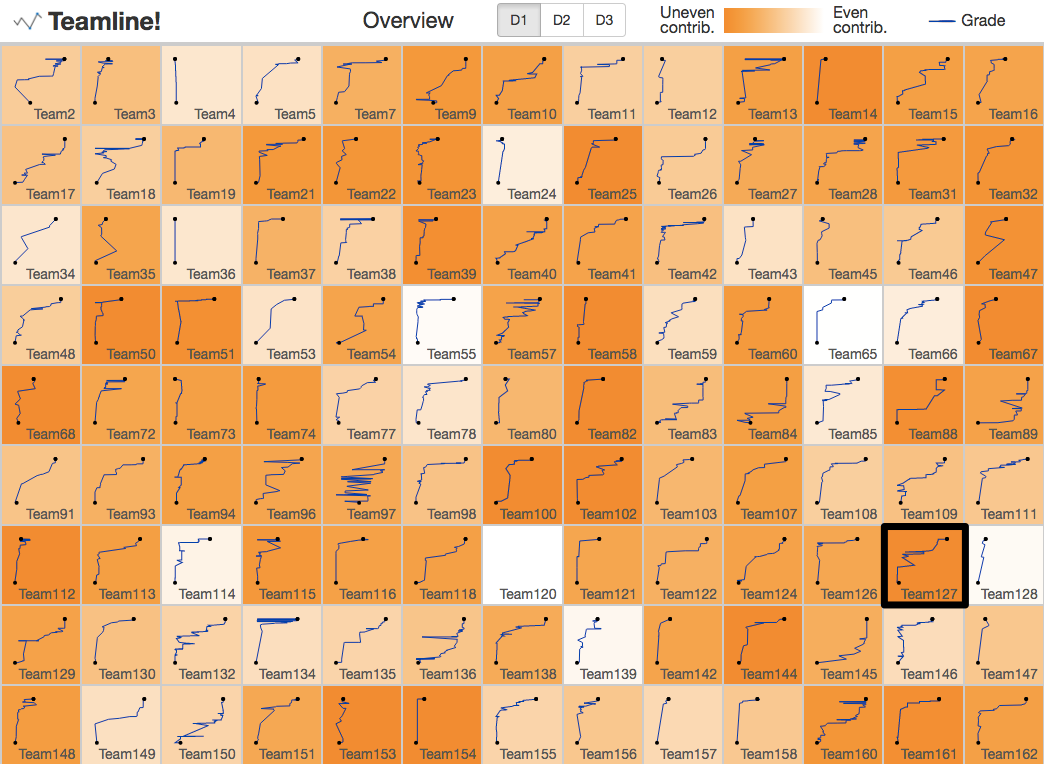
\includegraphics[width=\linewidth]{sample-overview}
  \caption{Sample overview}
  \label{fig:sample-overview}
\end{figure}

\begin{figure}[h]
  \centering
  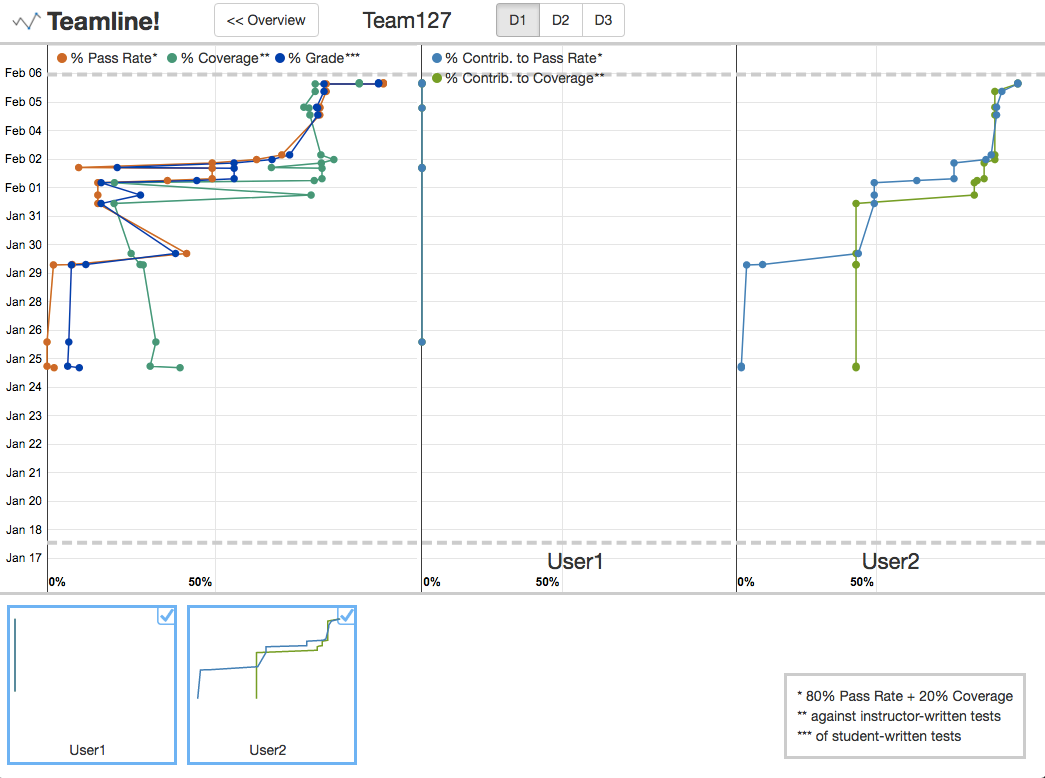
\includegraphics[width=\linewidth]{sample-teamview}
  \caption{Sample team view for Team127}
  \label{fig:sample-teamview}
\end{figure}



% \begin{table}
%   \label{tab:analysis}
%   \caption{What-Why-How analysis of Teamline.}
%   \begin{tabularx}{\columnwidth}{ l | l }
%     \hline
%     What: Data & Table of graded commits. \\
%     What: Derived & \parbox{6cm}{Measure of contribution to pass rate and coverage. Contribution uniformity.}  \\
%     Why: Tasks & \parbox{6cm}{Present the uniformity of contributions and summarize the team's commit history.} \\
%     How: Encode & \parbox{6cm}{We used a heatmap in the overview with}  \\
%     How: Facet & \parbox{6cm}{Overview + detail views. Detail view is partitioned into side-by-side views.} \\
%     How: Embed & \parbox{6cm}{Superimpose sparklines on the overview's heatmap cells.} \\
%     How: Reduce & \parbox{6cm}{Filtering is done by selecting the team and the deliverable in}  \\
%     \hline
%   \end{tabularx}
% \end{table}



% \begin{table}[h!]
%   \centering
%   \caption{Caption for the table.}
%   \label{tab:table1}
%   \begin{tabular}{l|c||r}
%     1 & 2 & 3\\
%     \hline
%     a & b & c\\
%   \end{tabular}
% \end{table}

\end{document}
